\documentclass[14pt, a4paper]{extreport}
\usepackage{susu}

% ====================================================================================================
\begin{document}

\author{Новгородцев~Н.В.}
\group{211}
\task{3}
\maketitle

% ====================================================================================================
\chapter{Задание}

\begin{enumerate}

	\item
	Привести описание и схему алгоритма Ву для растрового представления линии.

	\item
	Разработать подпрограмму для рисования линии (аналог процедуры line из графической библиотеки). Аргументы подпрограммы – координаты 				начальной и конечной точек. При реализации подпрограммы использовать для рисования только процедуру putpixel. Для определения текущего 			цвета рисования использовать функцию getcolor.

	\item
	Разработать подпрограмму для рисования правильной звезды. Аргументы подпрограммы – координаты центра, радиус описанной окружности и 			число вершин. При создании контура звезды использовать собственную подпрограмму рисования линии. Для закраски фигуры использовать 				процедуру floodfill.

	\item
	Написать программу для тестирования разработанных подпрограмм. Интерфейс программы должен содержать следующие элементы управления:
	\begin{itemize}
		\item увеличение/уменьшение числа вершин;
		\item увеличение/уменьшение размера (радиуса описанной окружности);
		\item сохранение результата в файл;
		\item выход из программы.
	\end{itemize}

\end{enumerate}

% ====================================================================================================
\chapter{Математическая модель}

Пусть $x_0$, $y_0$, $x_1$, $y_1$ -- соответственно координаты первой и второй точки.
При рисовании линии цвет задан изначально $color$ в формате RGB и будем говорить что он равет col, а координаты простовляемого пикселя x и y.\\
Отрисовка линии:
$$ deltax = |x_1-x_0| . $$
$$ deltay = |y_1-y_0| . $$
$$ error = 0 . $$
$$ deltaerr = 0 . $$
Если deltay > deltax, то:\\
Если deltay не равно 0 то:
$$ deltaerr = dx/dy . $$
Если $y_0$ > $y_1$, то меняем точки местами.
$$ x = x_0 . $$
$$ dir = x_1-x_0 . $$
\begin{equation*}
dir =
\left\{
\begin{array}{lr}
1 & \text{ для } dir > 0 \\
-1 & \text{ для } dir \leq 0
\end{array}
\right.
\end{equation*}
Потом перебераем все значения y от $y_0$ до $y_1$:\\
Ставим пиксель в координах x y и с цветом color.
$$ error = error+deltaerr . $$
Если error $\geq$ 1:
$$ x = x+dir. $$
$$ err = err-1. $$
Если deltay $\geq$ deltaч, то делаем анологичные действия меняя в обработке x на y и y на x\\

Отрисовка звезды:\\
Пусть x и y центр звезды, r и n радиус внешной окружности и количество внешних углов.
$$ kof = \frac{cos(3.14/n*2)}{cos(3.14/n)} . $$
Перебираем каждый угол, где i это номер угла от 0 до 2n-1 включительно.\\
Если i чётное то:
$$ x_{i} = x+r*cos(i*3.14/n) . $$
$$ y_{i} = y+r*sin(i*3.14/n) . $$
Иначе:
$$ x_{i} = x+r*kof*cos(i*3.14/n) . $$
$$ y_{i} = y+r*kof*sin(i*3.14/n) . $$
После чего проводятся последовательные линии между точками(углами).

% ====================================================================================================
\chapter{Текст программы}

\noindent Файл main.cpp
\lstinputlisting{source/main.cpp}
\pagebreak
\hrulefill

\noindent Файл task.h
\lstinputlisting{source/task.h}
\hrulefill

\noindent Файл task.cpp
\lstinputlisting{source/task.cpp}
\hrulefill

\noindent Файл control.h
\lstinputlisting{source/control.h}
\hrulefill

\noindent Файл control.cpp
\lstinputlisting{source/control.cpp}

% ====================================================================================================
\chapter{Результат работы}

\begin{figure}[h!]
	\centering
	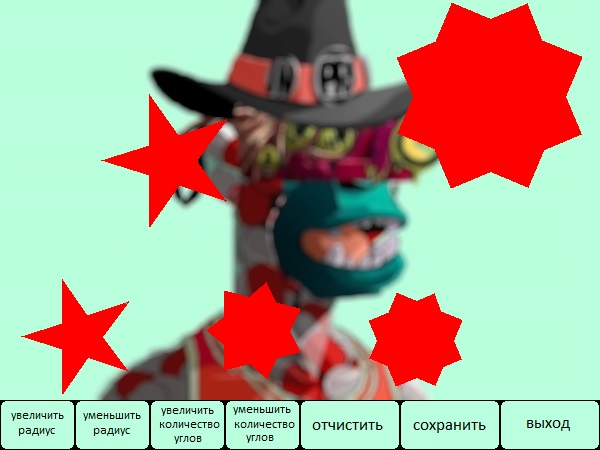
\includegraphics[width = 12cm]{image/image}
  \caption{Результат выполнения программы (Пример 1)}
\end{figure}


% ====================================================================================================
\end{document}